\section{Reference Model}
\begin{frame}\frametitle{Reference Architecture}
	\begin{itemize}
		\item Initially Reference architecture
		\begin{itemize}
			\item 4+1 view model
			\begin{itemize}
				\item Component / Package Diagram - Development View
				\item Class / State Diagrams - Logical view
				\item Deployment Diagram - Physical View
				\item Activity / Sequence Diagrams - Process View
				\item Use Cases - Scenarios
			\end{itemize}
		\end{itemize}
	\end{itemize}
	\begin{itemize}
		\item<2> Impossible with the given, not given constraints
	\end{itemize}
\end{frame}
\begin{frame}\frametitle{Reference Model}
	\begin{itemize}
		\item Single Model
	\end{itemize}
	\begin{itemize}
		\item Abstract
		\begin{itemize}
			\item Without changes cater to as many problems as possible
		\end{itemize}
		\item Flexibility
		\begin{itemize}
		\item Allow changes if needed
	
		\end{itemize}
	\end{itemize}
\end{frame}
\begin{frame}\frametitle{Reference Model}
	\begin{figure}
		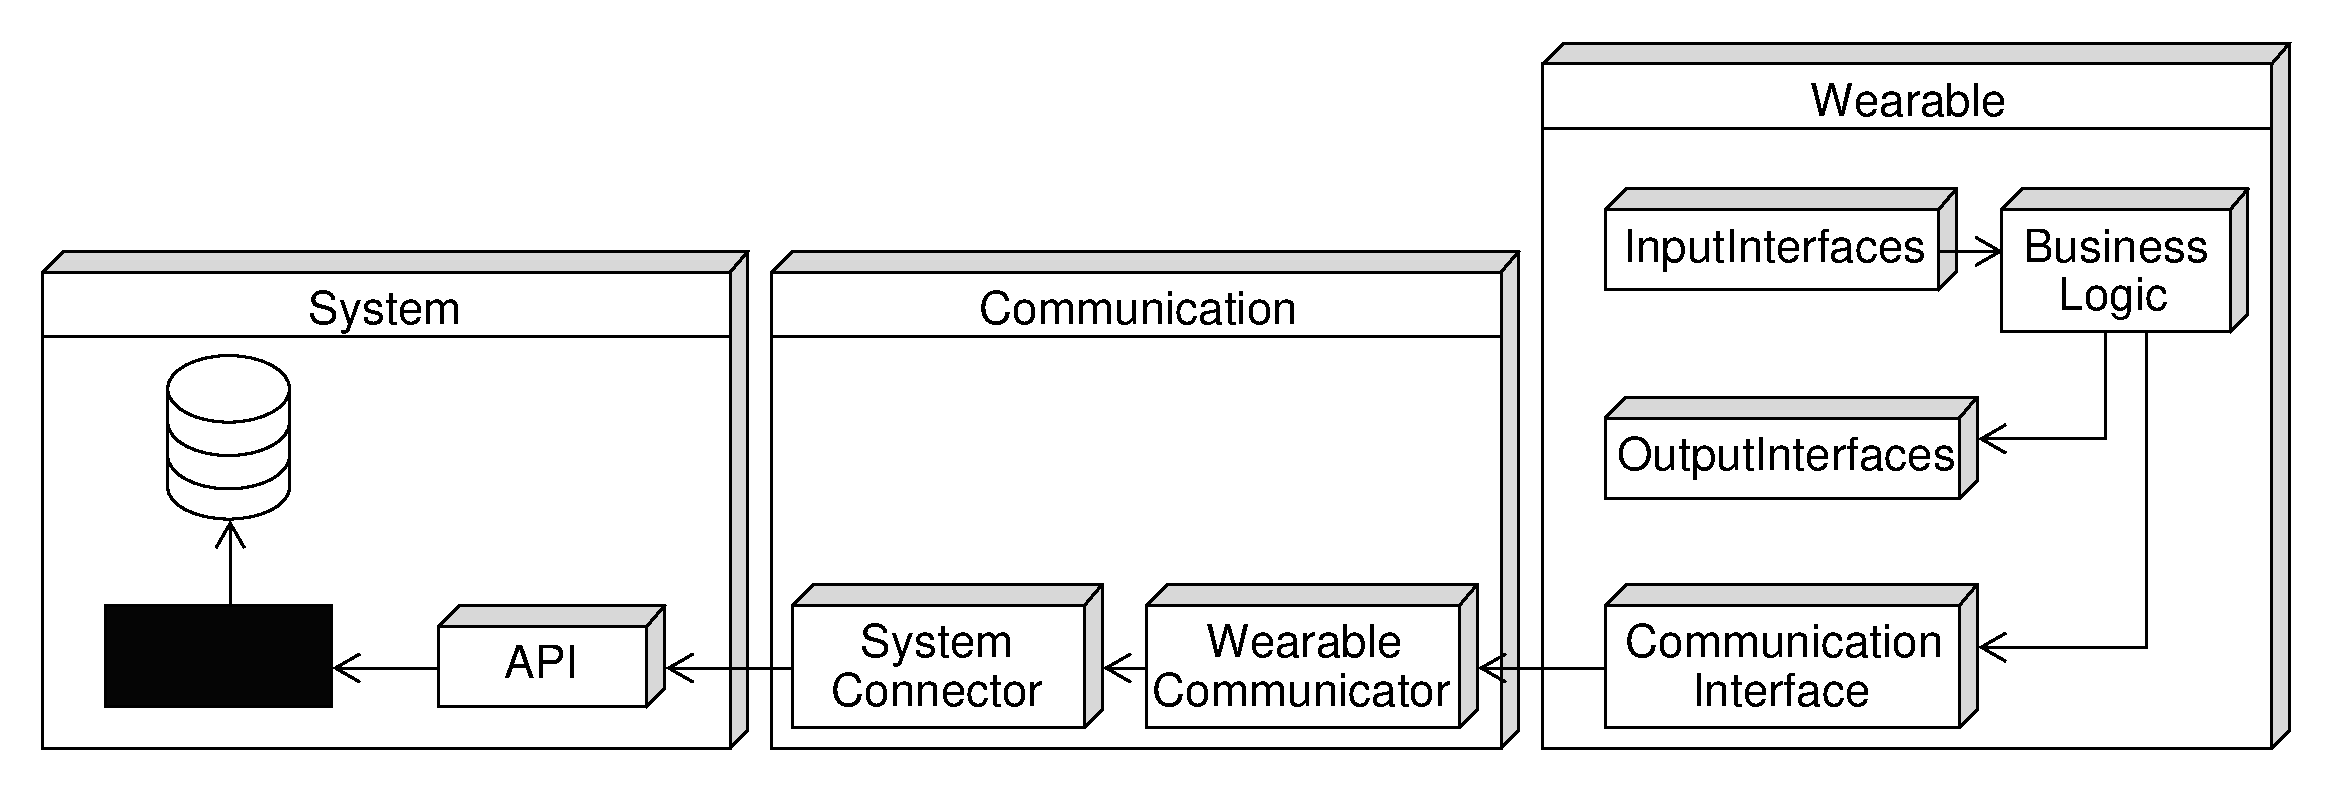
\includegraphics[width=\textwidth]{images/ReferenceModel}
	\end{figure}
\end{frame}
\begin{frame}\frametitle{Reference Model Examples}
	\begin{figure}
		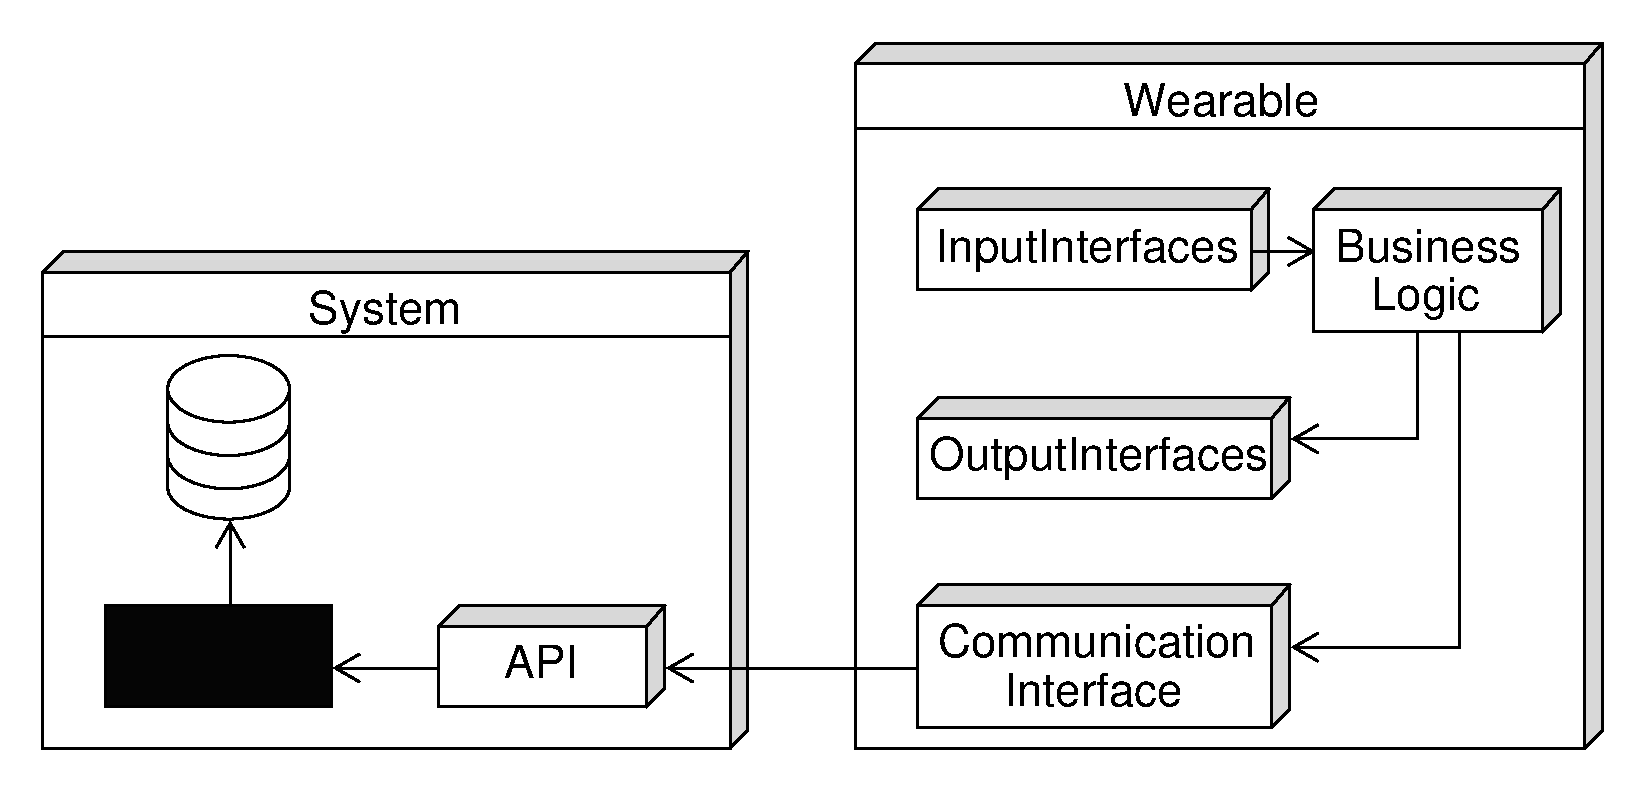
\includegraphics[width=\textwidth]{images/ReferenceModel_NoCommunication}
	\end{figure}
\end{frame}
\begin{frame}\frametitle{Reference Model Examples}
	\begin{figure}
		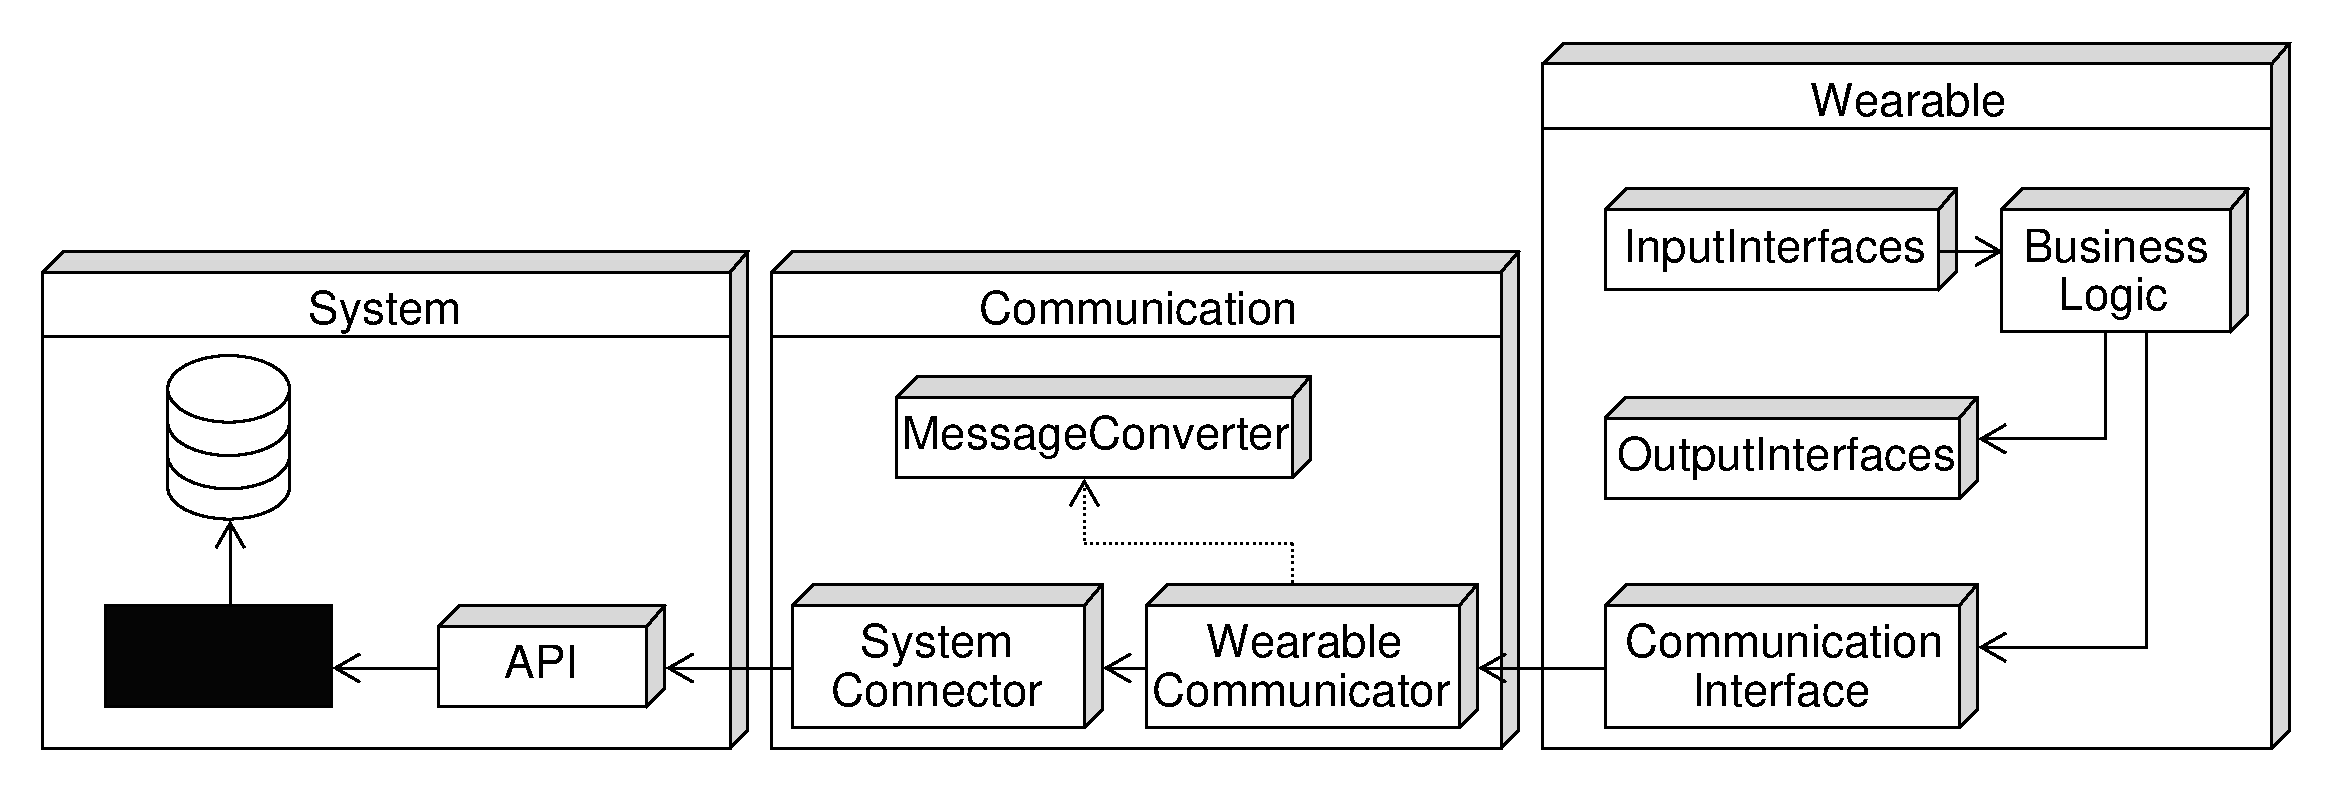
\includegraphics[width=\textwidth]{images/ReferenceModel_Converter}
	\end{figure}
\end{frame}